% =========================================================
% Physics Letters B — Elsevier 2-column (elsarticle, 5p)
% =========================================================
\documentclass[final,5p,times,authoryear]{elsarticle}
% options:
%   final,5p,times      -> two-column journal look
%   preprint,12pt       -> single-column review copy
%   (swap authoryear -> numeric by changing \bibliographystyle)

% ---------- Packages compatible with Elsevier ----------
\usepackage[T1]{fontenc}
\usepackage[utf8]{inputenc}
\usepackage{amsmath,amssymb,bm}
\usepackage{graphicx}
\usepackage{booktabs}
\usepackage{siunitx}
\usepackage[hidelinks]{hyperref}
\usepackage[nameinlink,capitalize]{cleveref}
% \usepackage{lineno}   % uncomment + \linenumbers after \end{frontmatter} if needed

\sisetup{
  mode = match,
  propagate-math-font = true,
  text-family-to-math = true,
  text-series-to-math = true
}

\journal{Physics Letters B} % shows in footer when appropriate

\begin{document}

% ---------- OPTIONAL GRAPHICAL ABSTRACT / HIGHLIGHTS ----------
% Place BEFORE \begin{frontmatter}. Comment out if not used.
% \begin{graphicalabstract}
% \includegraphics[width=\textwidth]{grabs} % file 'grabs.pdf/png' if journal requires it
% \end{graphicalabstract}
% \begin{highlights}
% \item Key result in one line.
% \item Gate + threshold and outcome.
% \end{highlights}

\begin{frontmatter}

\title{Title of paper}

\author[neu]{Justin K.\ Lietz\corref{cor1}}
\address[neu]{Neuroca, Inc.}
\cortext[cor1]{Corresponding author.}
\ead{justin@neuroca.ai}

\begin{abstract}
Example abstract for \textit{Physics Letters B}. Provide a brief summary of the research
and results in $\le$200 words.
\end{abstract}

\begin{keyword}
reaction–diffusion \sep metriplectic \sep reproducibility \sep scaling
\end{keyword}

\end{frontmatter}
% \linenumbers

% ====================== 1. INTRODUCTION ======================
\section{Introduction}
Here is where you provide an introduction to work and some
background. For example building on previous work of im-
age enhancment in optical astronomy \citep{Fortunato2010}. \citet{Vehlowetal2013} developed a method to improve the reso-
lution of X-ray images from XMM-Newton to provide similar
spatial resolution to Chandra. State exactly what is and is not claimed.

% ====================== 2. TITLE 2 ===========================
\section{Title 2}
Lorem ipsum dolor sit amet, consectetuer adipiscing elit. Ut
purus elit, vestibulum ut, placerat ac, adipiscing vitae, felis.
Curabitur dictum gravida mauris. Nam arcu libero, nonummy
eget, consectetuer id, vulputate a, magna. Donec vehicula au-
gue eu neque. Pellentesque habitant morbi tristique senectus et
netus et malesuada fames ac turpis egestas. Mauris ut leo. Cras
viverra metus rhoncus sem. Nulla et lectus vestibulum urna
fringilla ultrices. Phasellus eu tellus sit amet tortor gravida pla-
cerat. Integer sapien est, iaculis in, pretium quis, viverra ac,
nunc. Praesent eget sem vel leo ultrices bibendum. Aenean
faucibus. Morbi dolor nulla, malesuada eu, pulvinar at, mol-
lis ac, nulla. Curabitur auctor semper nulla. Donec varius orci
eget risus. Duis nibh mi, congue eu, accumsan eleifend, sagittis
quis, diam. Duis eget orci sit amet orci dignissim rutrum.

\subsection{Subsection title}
Toomre stability criterion example:
\begin{equation}
  Q=\frac{\sigma_v\,\kappa}{\pi\,G\,\Sigma}.
\end{equation}

% ====================== 3. TITLE 3 ===========================
\section{Title 3}
One regular-width figure (fits one column):

\begin{figure}[!t]
  \centering
  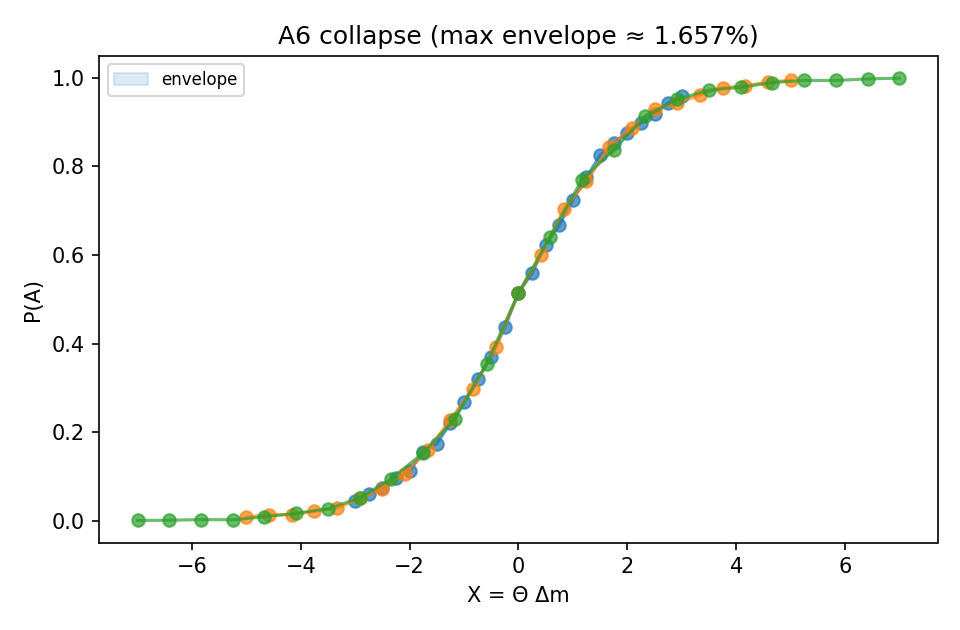
\includegraphics[width=\linewidth]{fig_1} % match your file name/case (fig_1.png/pdf)
  \caption{Example figure caption in Elsevier two-column format.}
  \label{fig:plbcover}
\end{figure}

% For a figure spanning BOTH columns, use the star form:
% \begin{figure*}[!t]
%   \centering
%   \includegraphics[width=0.95\textwidth]{fig_wide}
%   \caption{Wide figure spanning both columns.}
%   \label{fig:wide}
% \end{figure*}

\subsection{Subsection title}
Additional text…

% ====================== 4. DISCUSSION ========================
\section{Discussion}
Interpretation tied to figures/tables; keep claims bounded by data.

% ====================== 5. SUMMARY AND CONCLUSIONS ===========
\section{Summary and conclusions}
Short, testable summary.

\section*{Acknowledgements}
Thanks to …

\appendix
\section{Appendix title 1}
Appendix text.

\section{Appendix title 2}
Appendix text.

% -------------------------- References -----------------------
% Author–year like PLB sample:
\bibliographystyle{elsarticle-harv}
\bibliography{references}

% For numeric style instead, swap to:
% \bibliographystyle{elsarticle-num}         % and remove 'authoryear' from \documentclass

\end{document}
